\documentclass{standalone}
\usepackage{tikz}
\usepackage{ctex,siunitx}
\setCJKmainfont{Noto Serif CJK SC}
\usepackage{tkz-euclide}
\usepackage{amsmath}
\usetikzlibrary{patterns, calc,3d}
\usetikzlibrary {decorations.pathmorphing,decorations.pathreplacing,decorations.shapes}
\begin{document}
\small
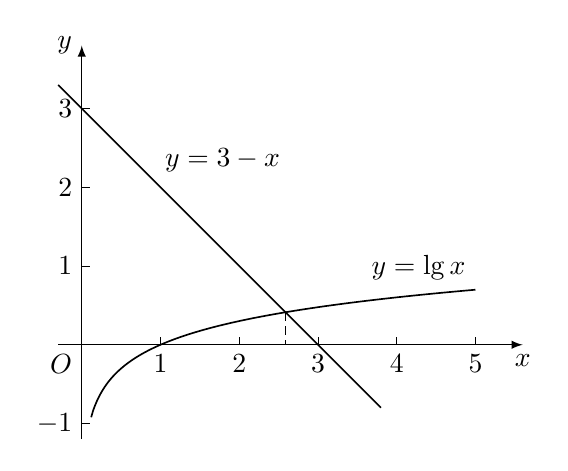
\begin{tikzpicture}[>=latex,scale=1.0]
  \draw[->](-0.3,0)--(5.6,0)node[below]{$x$};
  \draw[->](0,-1.2)--(0,3.8)node[left]{$y$};
  \node at (0,0)[below left]{$O$};
  \draw[semithick](3.8,-0.8)--(-0.3,3.3)node[pos=0.7,above right]{$y=3-x$};
  \foreach \x in {1,2,3,4,5} {\draw[very thin](\x,0)node[below]{$\x$}--++(0,0.1);}
  \foreach \x in {1,2,3,-1} {\draw[very thin](0,\x,0)node[left]{$\x$}--++(0.1,0);}
  \draw[semithick,samples=200,domain=0.12:5]plot(\x,{log10(\x)})node[above left]{$y=\lg x$};
  \draw[densely dashed](2.59,0.41)--(2.59,0);
\end{tikzpicture}
\end{document}